\chapter{Epílogo: Aventuras Finales y Despedida}
\vspace{0.6cm}
\begin{center}
\nopagebreak
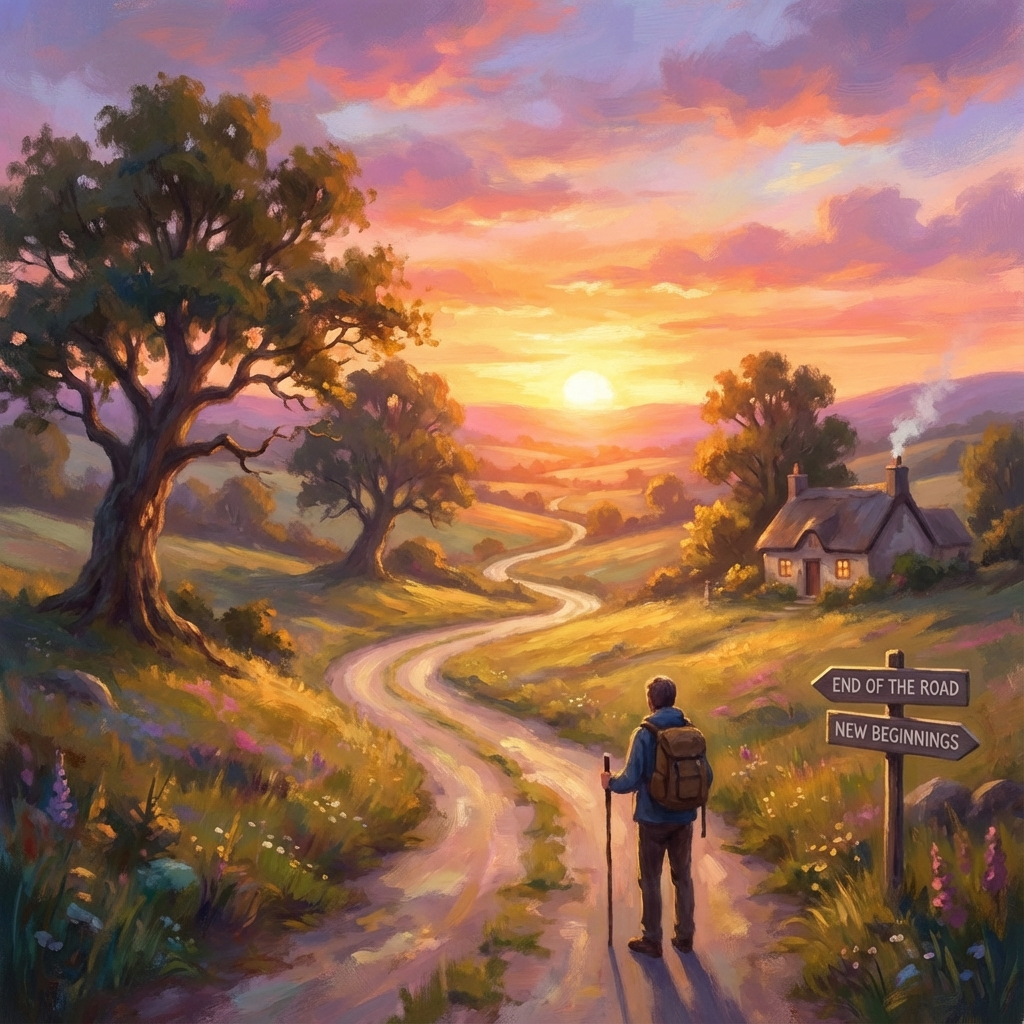
\includegraphics[width=0.75\textwidth,cfbox=gray!60 0.6pt 4pt]{sunset_road.png}\\
\vspace{4pt}
{\small\itshape El atardecer en el camino: la caminata del alma continúa.}
\end{center}

\vspace{0.6cm}
Jesús se despidió de mí en la estación de Atocha. Iba a coger un tren, dijo, hacia ninguna parte y hacia todas partes.
—¿Volveré a verte? —pregunté, sintiendo un nudo en la garganta.

—Siempre me ves —sonrió—. Estoy en la sonrisa del cajero del supermercado. En el viento que mueve los árboles de Colmenarejo. En el silencio de tu habitación. Pero sobre todo, estoy en ti. Cuando vibras alto, cuando amas, cuando perdonas... ahí estoy yo. Ahí somos uno.

Me dio un abrazo fuerte. Olía a madera y a lluvia fresca.
—No nos dejes caer en tentación —me susurró al oído—. Mantén la frecuencia, amigo. Mantén la música sonando. Y si alguna vez desafinas, no te juzgues. Simplemente, vuelve a sintonizar.

Se dio la vuelta y se mezcló con la multitud. Lo vi alejarse, con sus vaqueros y su caminar tranquilo, entre gente que corría mirando sus móviles. Y por un momento, me pareció ver que todo el vestíbulo de la estación brillaba con una luz dorada.

Salí a la calle. Madrid seguía igual: ruidosa, caótica, viva. Pero yo ya no era el mismo. Respiré hondo, sentí el sol en la cara y sonreí. Estaba vibrando alto. Y supe que, pasara lo que pasara, todo iba a estar bien.

\textbf{Fin.}